%! Author = vojmo
%! Date = 29.01.2022

\chapter{Analýza}

\section{Kvalitativní průzkum}

%TODO: Popsat více?
Nejprve bylo potřeba zjistit, co by potenciální uživatelé aplikace ocenili, tedy získat od nich požadavky.
Zvolili jsme kvalitativní průzkum, který se narozdíl od kvantitativního zamřuje na malou skupinu respondentů.
Pro získání odpovědí jsem si připravil sadu otevřených otázek, kterých jsem se držel při rozhovoru. Hovory byly
uskutečněny online a každy trval mezi dvaceti minutami a jednou hodinou.

Všechny rozhovory byly vedeny v rozmezí dvou týdnů a poté jsem z nich sestavil funkční a nefunkční požadavky.

\section{Funkční požadavky}

\subsection{F1: Správa receptů}
Pro uživatele je důležité udržovat své recepty aktuální. Je tedy nutné implementovat rozhraní, které umožní pracovat s
přidanými recepty.
\subsection{F2: Sdílení receptů}
Narozdíl od ostatních služeb, které jsou popsány dále v textu, by tato měla poskytovat sdílení mezi uživateli. Na to se pojí i
viditelnost receptů, tedy všechny nebudou veřejné, ale bude možné je přidat jako soukromé či neveřejné.
\subsection{F3: Objednávky přes služby typu rohlik.cz}
Převážně mladší generace dnes hojně využívá služeb na rozvoz nákupu. Je tedy potřeba přidat zjednodušený přesun potřebných
surovin do nákupních košíků v těchto službách, a tak zefektivnit čas nákupu.
\subsection{F4: Plánovač}
Pro mnoho lidí je důležité naplánovat si kdy mají čas si jídlo uvařit a naopak kdy by ho potřebovali mít již hotové. Pro bude v
aplikaci plánovač, kde bude uživatel moci sledovat, kdy ho čeká co uvařit.
\subsection{F5: Správa spíže}
Tento požadavek souvisí s těmi předchozími, tedy hlavně ulehčí uživateli nákup surovin a plánování vaření. Pokud uživatel nebude chtít
kontrolovat jaké suroviny má doma, funkci nebude muset využít.
\subsection{F6: Možnost ankety kolem jídelníčku}
Spíše než v běžném životě by se anketa dala využít například při výletu s kamarády či soustředění s týmem nebo kapelou. Uživatelé
by měli možnost hlasovat, v jaký den a jaké jídlo by chtěli.

\section{Nefunkční požadavky}

\subsection{U1: Dostupné jako webová aplikace}
Vzhledem k potřebě mít aplikaci dostupnou jak pro mobily, tak pro počítač, je webová aplikace nejflexibilnější řešení.
\subsection{P1: Systém pro jednotky uživatelů}
Aplikaci nebude využívat mnoho uživatelů, ale je nutné myslet na budoucí rozšíření.
\subsection{S1: Serverless s možností připojení na speciální API v budoucnu}
Prozatím se pro backendovou část využije \emph{serverless} řešení. Pokud by tato alternativa v budoucnu neposkytovala dostatečné
funkce nebo se nevyplatila finančně, je možné přejít na jiný backend.

\begin{figure}[h]
    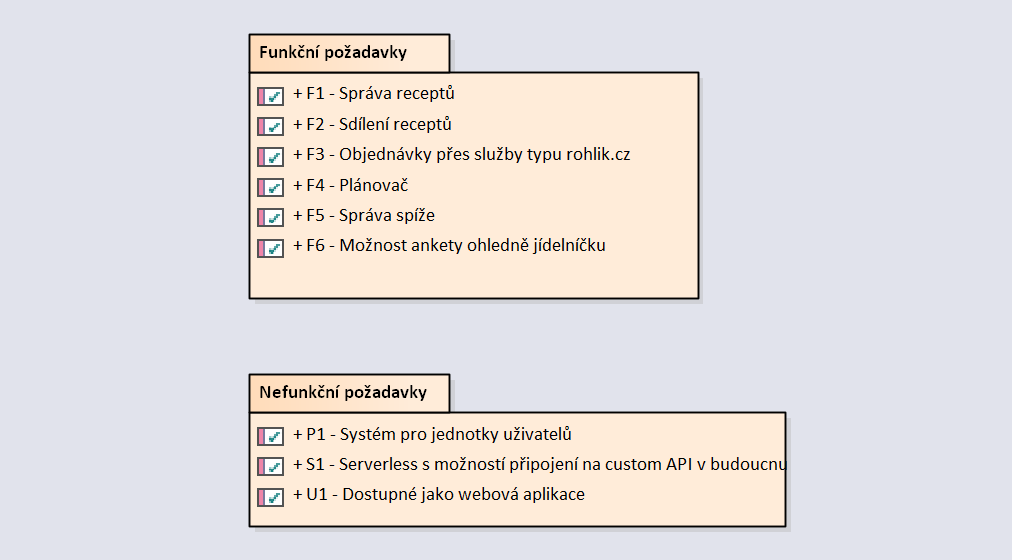
\includegraphics[width=\textwidth]{images/pozadavky}
    \caption{Model požadavků} \label{picture:recipeo:pozadavky}
\end{figure}

\section{Existující řešení}

Porovnal jsem nejpoužívanější české portály s recepty. Některé z nich nabízejí další obsah jako například blog či magazín.

\subsection{Vareni.cz}

Na vareni.cz~\cite{VareniCZ} se nachází několik reklam, které jsou velké a rušivé. Není zde možné si přidat soukromý recept a sdílet ho
pouze s vybranými uživateli. Celkový koncept přidání receptu je pouze veřejný, není tedy možné si zde vytvořit sbírku
oblíbených receptů z různých portálů. Vyhledávání je možné podle názvu, ingrediencí či různých parametrů jako je druh jídla
nebo národní kuchyně. Recepty mají hodnocení od jedné do pěti hvězdiček.

Na stránce konkrétního receptu je shrnutí nejdůležitějších vlastností, tedy název, krátký popis, hodnocení a čas vaření.
Také v hlavičce kolují různé komentáře. Výhodou jsou návrhy podobných receptů. Naopak velmi špatné je rozložení seznamu ingrediencí
a postupu přípravy. Tato část je velmi nepřehledná a je nerozeznatelné kde recept končí a začínají jiné recepty.

Jsou zde kuchařky, ale než že by byly tématické nebo měli společného autora, přišlo mi, že se jedná se o náhodnou kolekci receptů,
kde je jich často více než tisíc.

Celkem hezký nápad jsou fotorecepty. Uživatele provedou celým vařením pomocí kroků, přičemž u každého je fotodokumentace jak daný krok
provést.

\begin{figure}[h]
    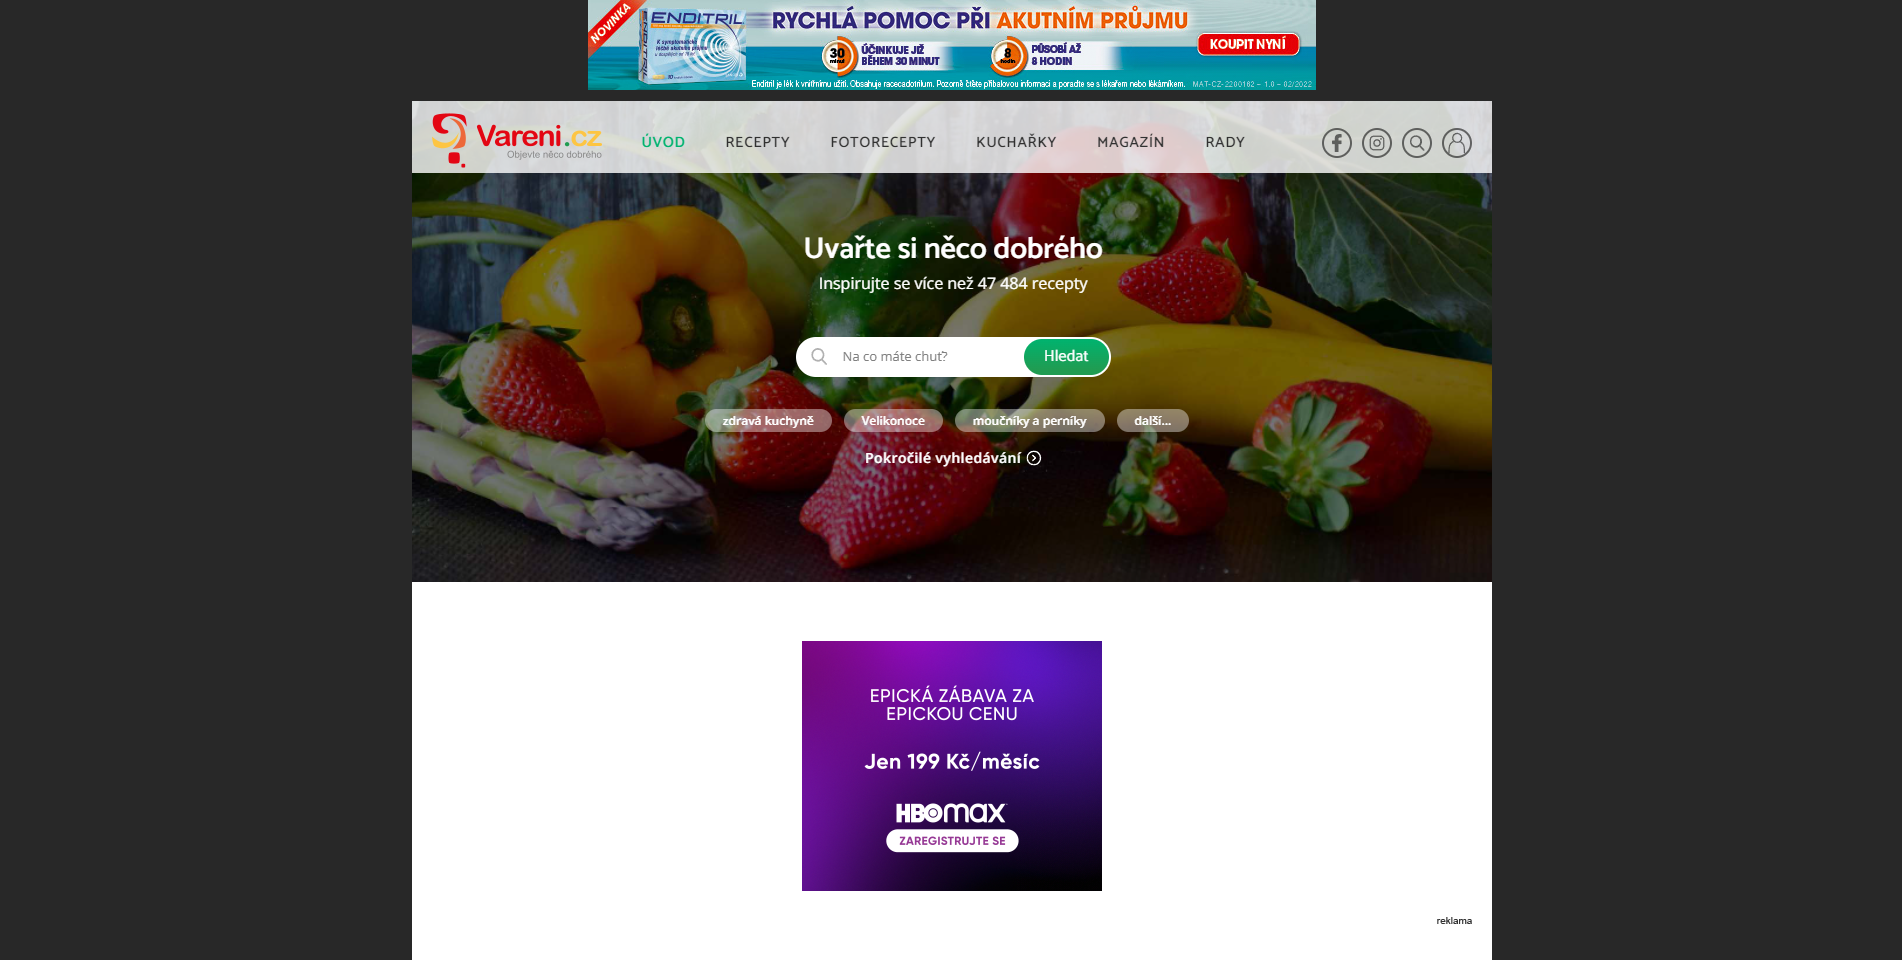
\includegraphics[width=\textwidth]{images/varenicz-uvodni-stranka}
    \caption{Hlavní stránka vareni.cz} \label{picture:varenicz:uvodni-stranka}
\end{figure}

\subsection{Toprecepty.cz}

Na tomto portálu~\cite{TopreceptyCZ} byla bohužel nefunkční registrace, takže jsem nemohl nahlédnout na funkce poskytované přihlášeným
uživatelům. Opět zde byla přítomna velká reklama, která zabírala většinu stránky. Jinak byl web navrhnut přehledně,
ale narazil jsem na několik nefunkčních prvků na mobilním zobrazení. Zhodnotit přidání receptů a jak funguje jejich
sdílení zhodnotit nemohu, kvůli výše zmíněným problémům. Našel jsem funkci podobnou doporučování receptů, avšak se
pravděpodobně jedná o náhodné doporučení, které nemá nic společného s tím co má uživatel rád. Dále je na webu dostupný
online magazín, kde jsou různé články týkající se gastronomie.

\begin{figure}[h]
    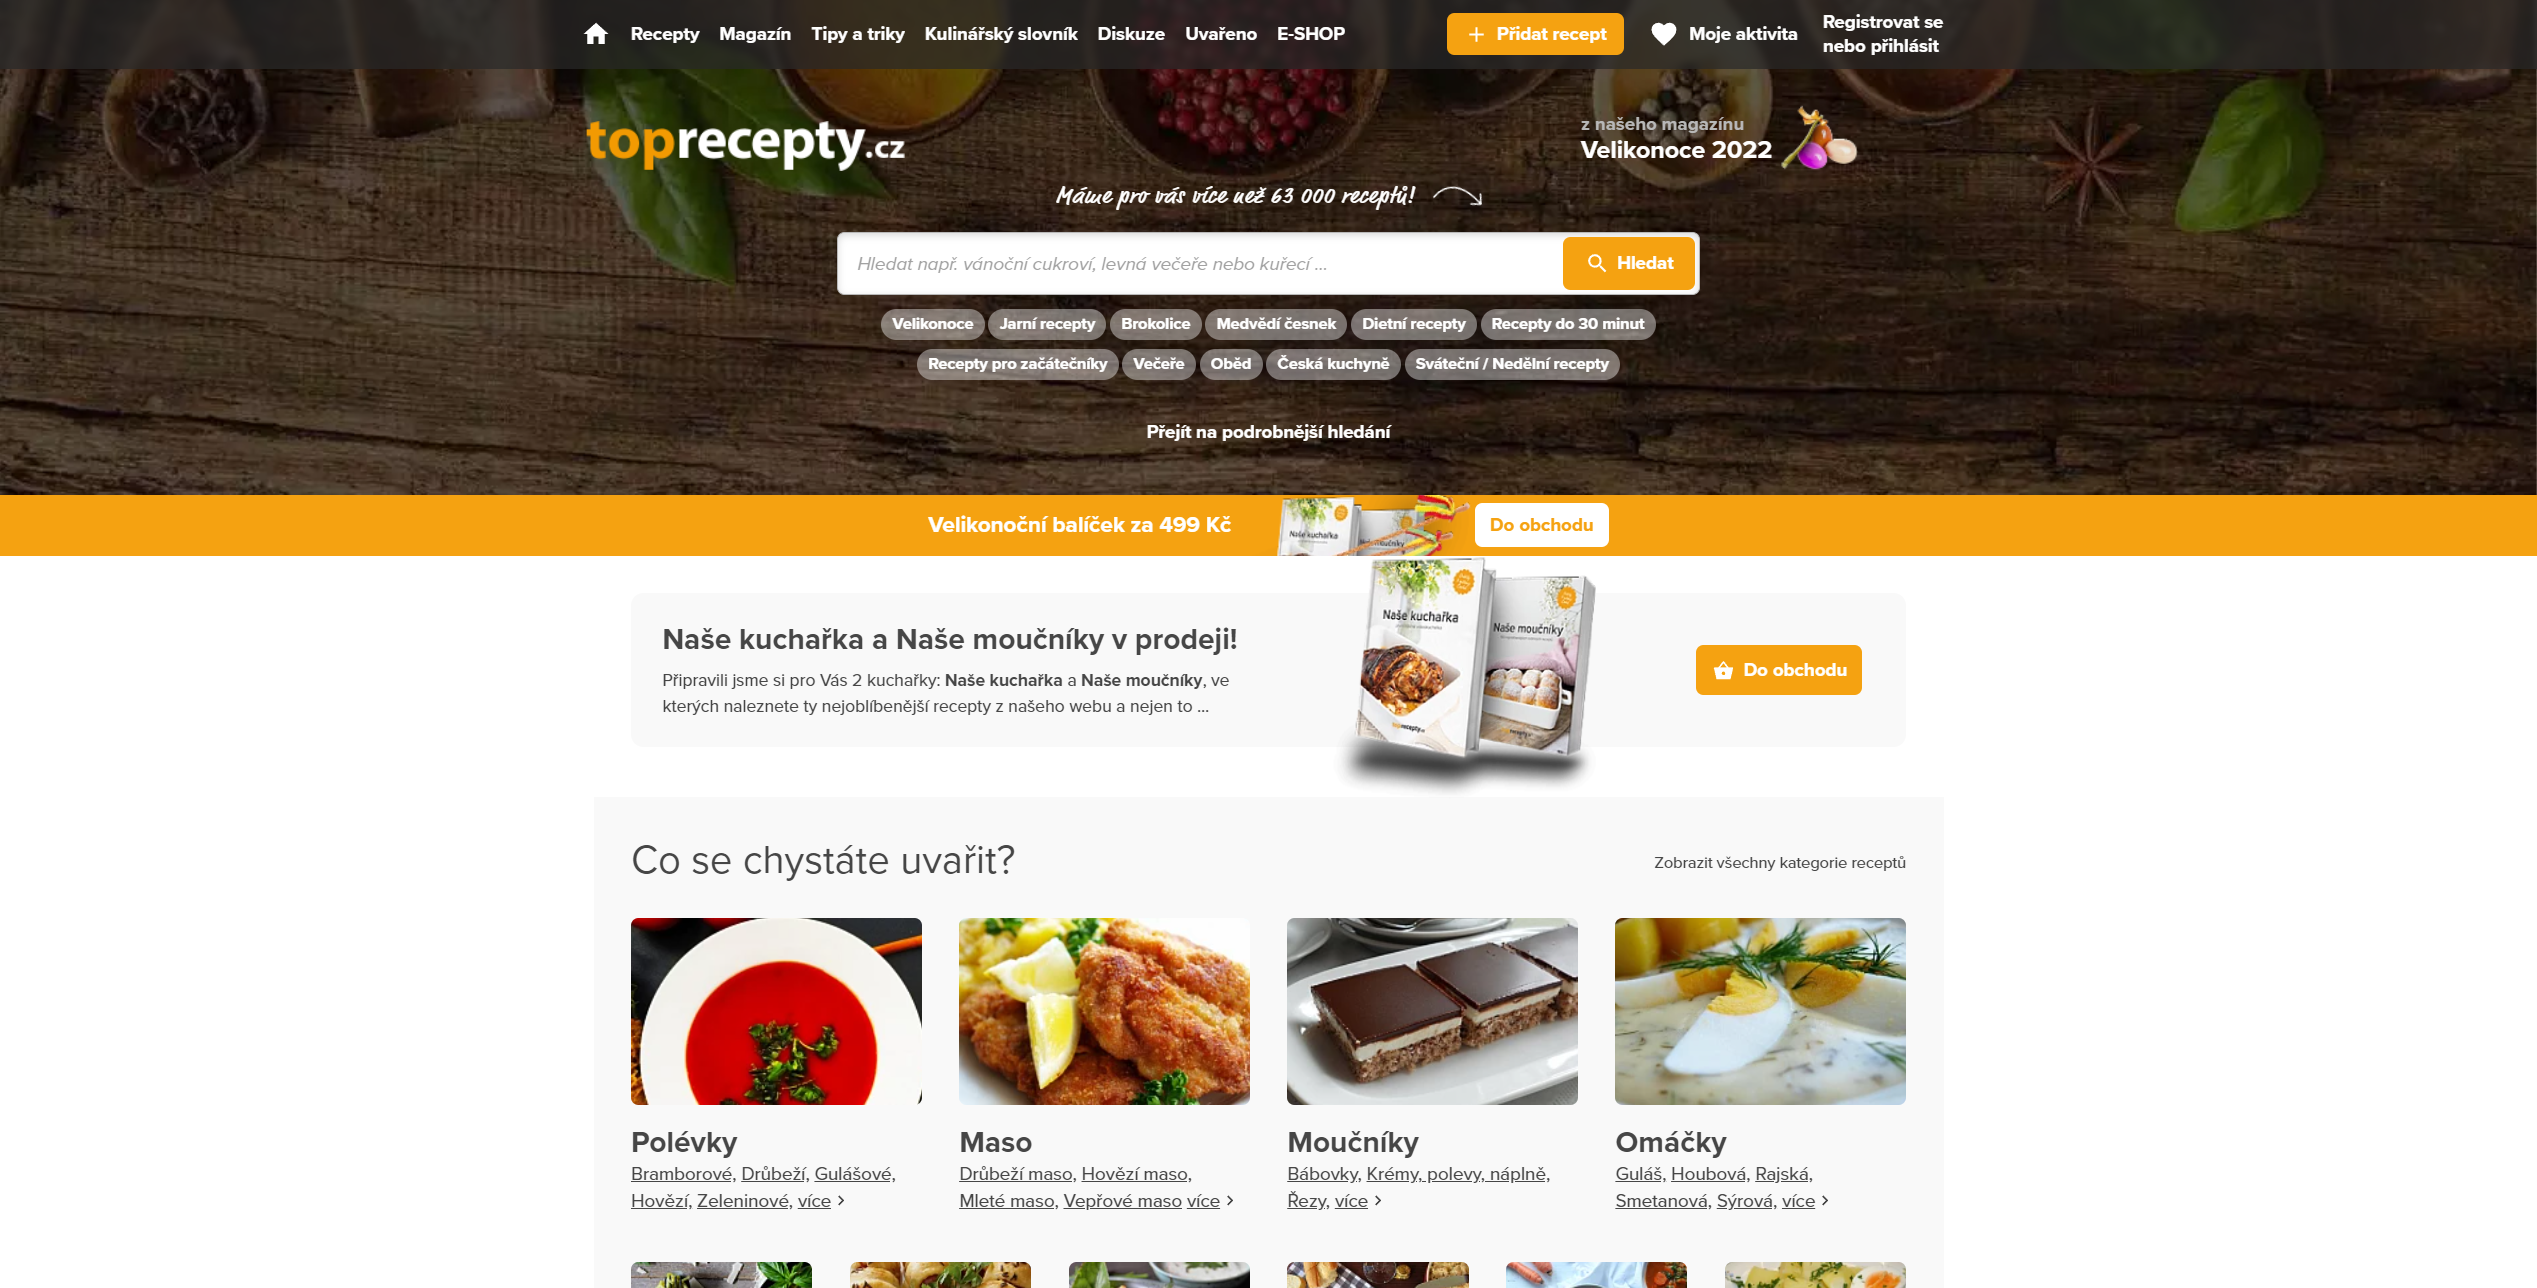
\includegraphics[width=\textwidth]{images/topreceptycz-uvodni-stranka}
    \caption{Hlavní stránka toprecepty.cz} \label{picture:topreceptycz:uvodni-stranka}
\end{figure}

\subsection{Recepty.cz}

I třetí zástupce~\cite{ReceptyCZ} existujících řešení používá reklamu přes celou stránku okolo jejího obsahu. Podobně jako toprecepty.cz
je zde magazín obsahující příspěvky na spoustu témat o vaření. U přidání receptu nebylo napsané, co se s receptem stane,
zda bude veřejný nebo se zobrazí pouze mě. Po kliknutí na tlačítko \uv{Uložit recept}, se zobrazila stránka s nadpisem
\uv{Recept čeká na schválení}. Nebylo tedy opět možné soukromé použití.

Zobrazení receptu je podobné tomu na vareni.cz, ale přijde mi více přehledné. U kroků se zobrazují rady, které ale
nemají s daným krokem nic společného, spíše odkazují na náhodné články či recepty.

\begin{figure}[h]
    \includegraphics[width=\textwidth]{images/receptycz-uvodni-stranka}
    \caption{Hlavní stránka recepty.cz} \label{picture:receptycz:uvodni-stranka}
\end{figure}

\subsection{Závěr}

Existující řešení na vyhledávání receptů nabízejí pouze veřejné recepty a mají spoustu reklam. Moje řešení bude poskytovat
možnost soukromé sbírky receptů a jejich sdílení s vybranými uživateli či pomocí odkazu.

\section{Nákup surovin}

Vedoucí práce již dříve používal aplikaci Zdravý stůl~\cite{ZdravyStul}. Tam bylo možné si jídlo objednat přes rohlik.cz (vložit do košíku).
Tudíž jsme chtěli tuto funkcionalitu zachovat a přidat možnosti jako například vytvoření objednávky u konkurence - kosik.cz
či zobrazení interaktivního nákupního listu.

\subsection{Komunikace s Rohlíkem a Košíkem}
Nejdříve jsme se rozhodli kontaktovat Rohlík. Po pár vyměněných e-mailech jsme obdrželi celou dokumentaci k jejich API,
které nám otevřelo spoutu možností i do budoucna. Například bychom mohli sledovat, jaké suroviny jsou právě ve slevě a
podle toho doporučovat jídla.

Od Košíku jsme dostali pozvání na schůzku, kde jsme si mohli prohlédnout i jejich kanceláře. Na schůzce jsme hned na začátku
zjistili, že API pro partnery narozdíl od Rohlíku ještě dostupné není (Rohlík na API pro partnery také teprve pracuje,
ale zatím jsme dostali přístup k API pro jejich aplikaci), ale už na něm pracují. Plánované období vydání je
první kvartál roku 2022. Pro jeho využití je však potřeba OAuth server, který zatím není dostupný. % TODO: Zjistit v lednu.
Jako alternativu jsme dohromady vymysleli link na přidání surovin přímo do košíku, ze kterého nakonec sešlo, protože jsme
poté objevili funkci \uv{Nákupní lístek}, kterou bychom mohli využít. Odeslali bychom seznam surovin a uživatel by si je poté
mohl vybrat přímo z nabídky na Košíku. Nakonec jsme zjistili, že by se Košíku hodilo rozrůst sbírku receptů a bylo by možné
pro uživatele naší aplikace nabínout jejich recepty Košíku, který by je následně odkoupil.
